\section{Lo Strato di Trasporto}
Lo strato di trasporto dello stack protocollare TCP/IP presenta caratteristiche quali:
\begin{itemize}
    \item Realizzazione di \textcolor{purple}{comunicazioni logiche} fra processi residenti su host diversi. Logiche perché i processi si comportano come se gli host fossero direttamente collegati, ingorando i dettagli infrastrutturali.
    \item Offrire servizi di trasporto (per l'appunto) allo strato applicativo, che possono essere:
        \begin{itemize}
            \item \textcolor{blue}{Sequenze di messaggi singoli};
            \item \textcolor{blue}{Sequenza continua di byte}.
        \end{itemize}
        L'applicazione manda i dati al livello di trasporto, nella forma richiesta per la consegna.
    \item Sfrutta i servizi dello strato di rete che si occupa della comunicazione tra host e il quale consegna i datagrammi all'host destinatario (e non al processo).
\end{itemize}

\begin{figure}[h]
    \centering
    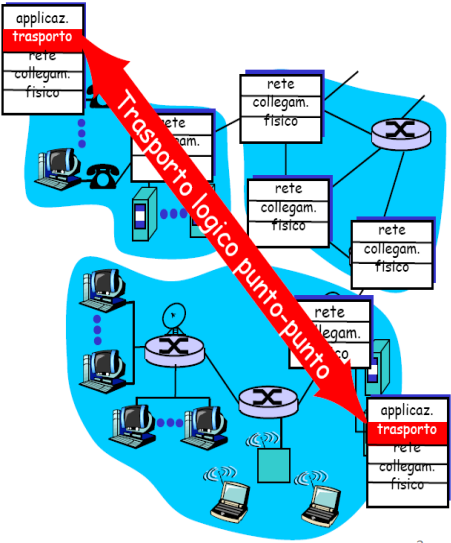
\includegraphics[scale=0.5]{Immagini/Lo_Strato_di_Trasporto.png}
    \caption{Lo strato di trasporto.}
\end{figure}

\newpage

\paragraph{Tipologie di Connessione}
Lo strato di trasporto offre principalmente due tipologie di servizio:
\begin{itemize}
    \item \textbf{\textcolor{purple}{Servizio privo di connessione:}} In questo caso il processo mittente di occupa di consegnare i \textcolor{blue}{messaggi} al livello di trasporto uno per uno e il livello di trasporto li considera in maniera indipendente, senza creare alcun tipo di relazione tra di essi. 
    \\In questa tipologia di servizio non vi sono garanzie di consegna o di ordinamento.
    \item \textbf{\textcolor{purple}{Servizio orientato alla connessione}} In questa tipologia di servizio il processo mittente e il processo destinazione vengono collegati mediante una \textcolor{blue}{connessione logica}.
\end{itemize}

I due principali protocolli messi a disposizione nel livello di trasporto, come detto nel capitolo precedente, sono TCP e UDP che vedremo poi in dettaglio.

\paragraph{Multiplexing e Demultiplexing}
Indipendentemente dal protocollo utilizzato, le azioni che vengono esequite durante le fasi di invio e ricezione dei segmenti sono le medesime:
\begin{itemize}
    \item Durante la fase di invio dei dati (\textcolor{purple}{Multiplexing}), il livello di trasporto riceve i messaggi dal livello applicativo, determina gli header per quel segmento, crea il segmento e invia il risultato al livello di rete (IP);
    \item Durante la fase di ricezione dei dati (\textcolor{purple}{Demultiplexing}), il livello di trasporto riceve i segmenti dal livello di rete, controlla i valori dell'header, estrae il messaggio e lo smista all'applicazione corretta attraverso la socket.
\end{itemize}

\paragraph{Concetto di Porta}
Ogni datagramma, presenta:
\begin{itemize}
    \item un indirizo IP sorgente e IP destinazione;
    \item un segmento del livello di trasporto, nel cui header sono presenti un numero di porta sorgente e un numero di porta destinazione.
\end{itemize}
Ogni comunicazione di trasporto è identificata in maniera univoca grazie alle coppie IP/porta degli host. Come visto in precedenza questi sono degli identificativi rispettivamente a 32 bit, per identificare l'host, e 16 bit, per identificare il processo sull'host. Il SO si occupa dell'assegnazione dinamica delle porte ai processi che ne fanno richiesta.
\\Esistono inoltre delle porte che sono assegnate arbitrariamente da IANA e che \underline{non} possono essere utilizzate liberamente dagli utenti o dalle applicazioni.

\paragraph{Demultiplexing con e senza connessione}
La fase di Demultiplexing dipende fortemente dal protocollo utilizzato. Nel caso del protocollo UDP le socket vengono identificate univocamente da una coppia IP/Porta, questo sta a significare che due datagrammi con IP e/o porta sorgente differenti ma medesima coppia IP/porta destinazione verranno consegnati alla stessa socket.

\begin{figure}[h]
    \centering
    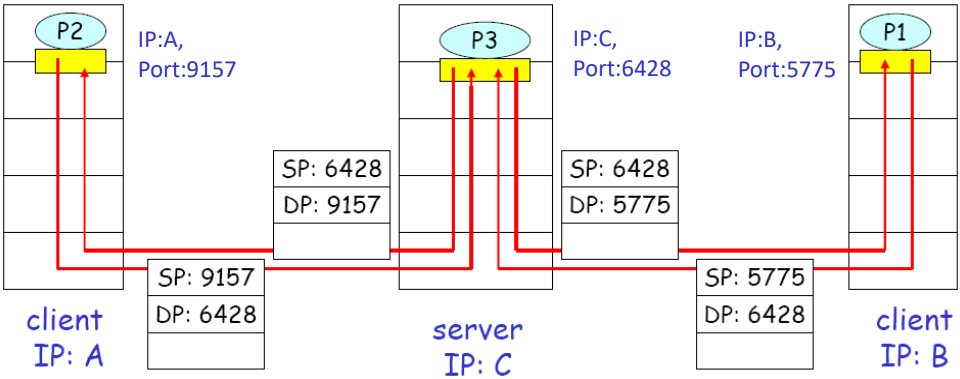
\includegraphics[scale=0.4]{Immagini/DemultiplexingUDP.png}
    \caption{Demultiplexing UDP.}
\end{figure}

Questo non è vero per le socket del protocollo TCP le quale vengono idetificate da una quadrupla data da:
\begin{itemize}
    \item Indirizzo IP di origine
    \item Numero di porta di origine
    \item Indirizzo IP di destinazione
    \item Numero di porta di destinazione
\end{itemize}
Una possibile consegnenza di ciò è che un host server può supportare più connessioni distinte contemporaneamente sulla stessa porta.

\begin{figure}[h]
    \centering
    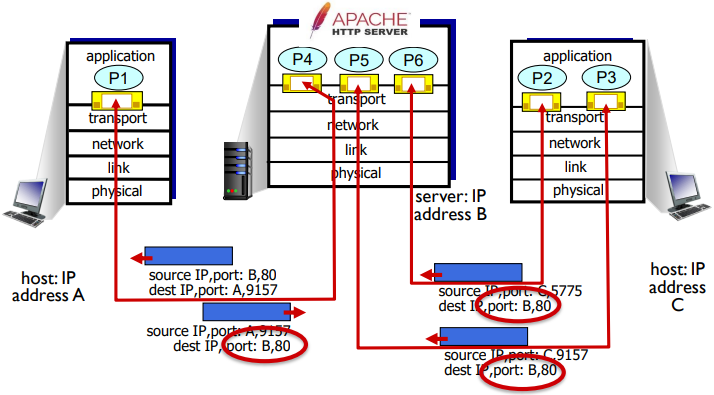
\includegraphics[scale=0.48]{Immagini/DemultiplexingTCP.png}
    \caption{Demultiplexing TCP.}
\end{figure}